\documentclass[12pt, a4paper]{article}
\usepackage[utf8]{inputenc}
 
\title{Exersice Sheet 1 (Solution)}
\author{Muhammad Fahad Bin Ashraf (412924), Shabi Turabi, Waleed Basit}
\date{May 2}

 % --- PACKAGES ---
\usepackage{pgfplots}
\pgfplotsset{width=10cm,compat=1.9}
\usepackage{graphicx}
\graphicspath{ {./images/} }
 
\usepackage{listings}
\usepackage{color}
\usepackage{amsmath , amssymb , amsthm}
\usepackage[utf8]{inputenc}

\definecolor{codegreen}{rgb}{0,0.6,0}
\definecolor{codegray}{rgb}{0.5,0.5,0.5}
\definecolor{codepurple}{rgb}{0.58,0,0.82}
\definecolor{backcolour}{rgb}{0.95,0.95,0.92}
 
\lstdefinestyle{mystyle}{
    backgroundcolor=\color{backcolour},   
    commentstyle=\color{codegreen},
    keywordstyle=\color{magenta},
    numberstyle=\tiny\color{codegray},
    stringstyle=\color{codepurple},
    basicstyle=\footnotesize,
    breakatwhitespace=false,         
    breaklines=true,                 
    captionpos=b,                    
    keepspaces=true,                 
    numbers=left,                    
    numbersep=5pt,                  
    showspaces=false,                
    showstringspaces=false,
    showtabs=false,                  
    tabsize=2
}
 
\lstset{style=mystyle}


\begin{document}
 
\begin{titlepage}
\maketitle
\end{titlepage}

\begin{enumerate}
    \item Identifying learning problems \\
    Part (a) and (b)
    \begin{itemize}
        \item Predictive maintenance:\\
        Data: large amount of irregular factory data \\
        Goal: to minimizes the risk of unexpected failures and reduces the amount of unnecessary preventive maintenance activities.
        humans can't do this task more accuratetely as Machines because its hard to manage billions of data without any automated or smart system.
        \item Customer support \\
        Data: large volume of customer data  (quantitative data, historical data) \\
        Goal: to improve chatbots and conversational interfaces for customer service.\\
        Human can do this task more better than any smart device because they can think of quick answers which machine cant do.
        \item Product recommendation \\
        Data: purchase history for a customer and a large inventory of products\\
        Goal: to identify those products in which that customer will be interested and likely to purchase.\\
        human cant do this task better than intelligent devices because its depend on the historical purchases which need to maintain all records manually.
    \end{itemize}
    AI/ML companies in Kaiserslautern:
    \begin{itemize}
        \item Deutsches Forschungszentrum für Künstliche Intelligenz (DFKI) \\
        The German Research Center for Artificial Intelligence (DFKI) was founded in 1988 as a non-profit public-private partnership. 
        It has research facilities in Kaiserslautern, Saarbrücken and Bremen, 
        a project office in Berlin, a Laboratory in Niedersachsen and a branch office in St. Wendel. 
        In the field of innovative commercial software technology using Artificial Intelligence, 
        DFKI is the leading research center in Germany.
        \item Insiders Technologies \\
        Insiders Technologies supports companies worldwide on their way to the digital transformation with 
        its intelligent software solutions based on Artificial Intelligence. More than 1,500 customers rely on Insiders’ 
        innovative solutions for intelligent input management and modern customer communication. 
        Insiders Technologies is your ideal partner for becoming a digital company.
        \item Digital Devotion \\
        The DDG – Digital Devotion Group® is dedicated to provide founders, scientists,investors and entrepreneurs with the best ecosystem 
        for developing digital business models with a focus on Cross Reality (AR/VR/MR), Blockchain (BC) and Artificial Intelligence (AI). 
        The ecosystem enables all partners and startups not only to present and test their innovations in e.g. virtual labs, b
        ut also to access clients, experts and know-how, the network and capital.
    \end{itemize}
    Visit to DFKI: \\ \\
    DFKI mission is to propel the utilization of human languages by machines and to make and improve IT-solutions that benefit by language use. 
    They direct propelled research in language innovation and give novel computational methods to processing text, speech and knowledge. 
    They take a stab at a more profound comprehension of human language and thought, concentrating the genuine needs of the end user and the requests of the market. 
    They create novel and upgraded solutions identified with data and knowledge management, content generation, and natural communication.
    \setcounter{enumi}{1}
    \item General equation is  w \(>\) x + b = 0 \\ 
    \begin{figure}[h]
        \centering
        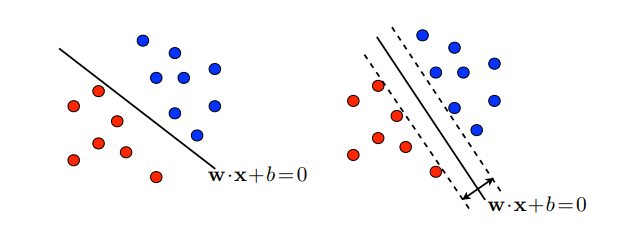
\includegraphics[width=8cm]{q2-img1}
    \end{figure}
    
    w \(\epsilon \) \(\mathbb{R}\) d is a non-zero normal vector \\
    
    b is a scalar intercept \\
    
    Divides the space in half, i.e. w \(>\) x + b \(>\) 0 and w \(>\) x + b \(<\) 0 \\
    
    A hyperplane is a line in 2D and a plane in 3D \\
    
    \begin{figure}[h]
        \centering
        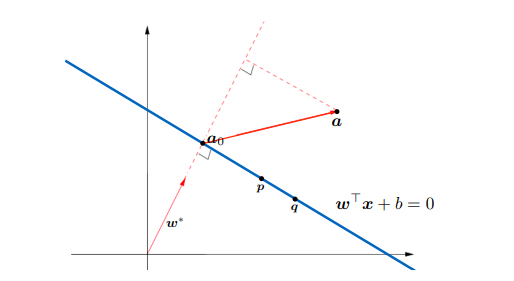
\includegraphics[width=8cm]{q2-img2}
        \caption{If two points, p and q are both on the line, then w \(>\) (p \(-\) q) = 0}
    \end{figure}

    p  \(-\) q is an arbitrary vector parallel to the line, thus w is orthogonal
    
    \(w_\ast = w \parallel w \parallel \) is the unit normal vector\\
    We want to find distance between a and line in direction of \(w_\ast\) \\
    If we define point \(a_0\) on the line, then this distance corresponds to length of \(a - a_0\)
    in direction of \(w_\ast\) , which equals \(w_\ast > (a - a_0)\)\\
    Since \(w>a_0 = -b\), the distance equals \( \frac{1}{\parallel w \parallel}(w^\top a + b)\)\\
    Similarly the signed distance from a point \(x^*\) to decision boundary (hyperplane) H is\\

    \(d(x^*, H) = \frac{w^\top x^* + b}{\parallel w \parallel}\)
    \pagebreak
	\item Distribution of weight and height among the citizens genders
	\begin{enumerate}
        \item Scatter plot
        \begin{figure}[h]
            \centering
            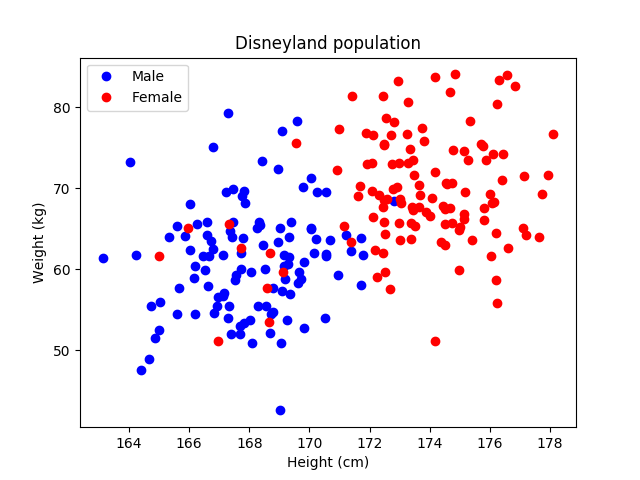
\includegraphics[width=10cm]{scatter_plot}
        \end{figure}
		\item Scatter plot with horizontal line to best seperate male and female citizens
        \begin{figure}[h]
            \centering
            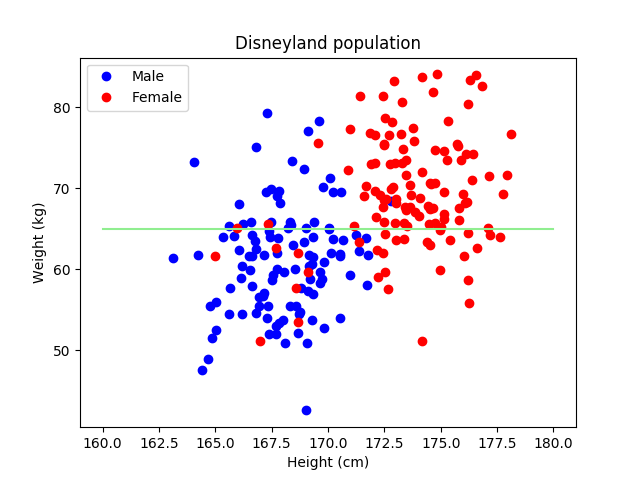
\includegraphics[width=10cm]{scatter_plot_line1}
        \end{figure}
		\item We would say that he/she is his father, but we cannot guarantee that because we do not know the hight value.
		\item Scatter plot with vertical line to best seperate male and female citizens
		\begin{figure}[h]
            \centering
            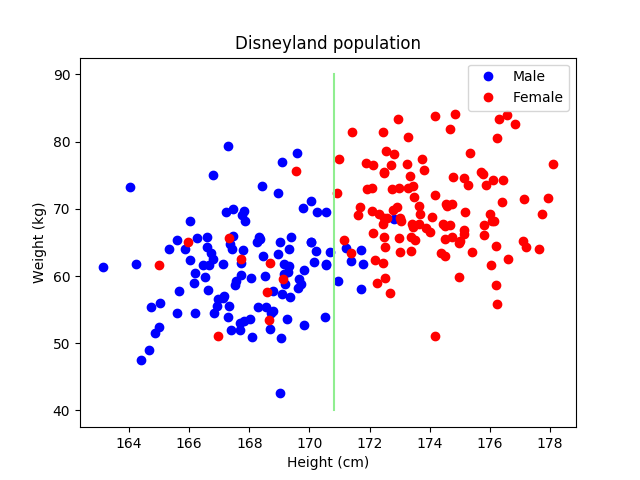
\includegraphics[width=10cm]{scatter_plot_line2}
        \end{figure}
        \item We would say that he/she is his sister, because according to the plot, almost all of the citizens 
        above the hight of 173 are females.
        \item Scatter plot with line to best seperate male and female citizens
		\begin{figure}[h]
            \centering
            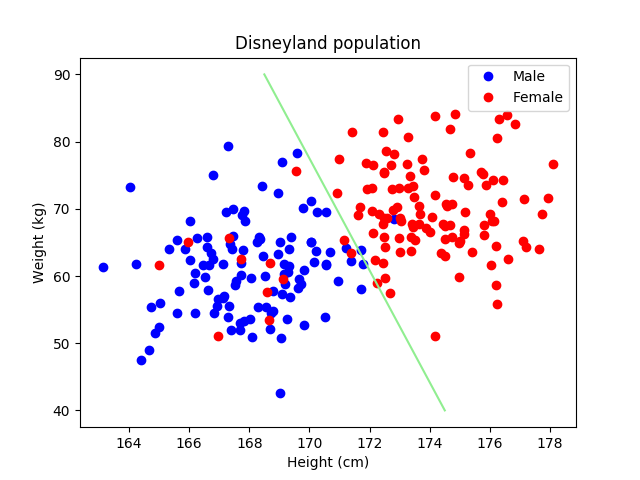
\includegraphics[width=10cm]{scatter_plot_line3}
        \end{figure}
        \item We would classify he/she as a "female" and no we would not classify 
        differently if we use (b) or (d) lines because all of the citizens in that area 
        are females.
    \end{enumerate}
    
    \setcounter{enumi}{4}
    \item k-nearest-neighbor learning algorithm
    \begin{enumerate}
        \item Algo implementation leaving 'k' as parameter
        \lstinputlisting[language=Python]{k-nn-algo.py}
        \newpage
        Output:
        \begin{figure}[h]
            \centering
            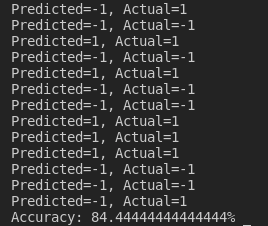
\includegraphics{k-nn-algo-output}
        \end{figure}
        \item k-fold cross validation algo show best avarage accuracy for k=5
        \lstinputlisting[language=Python]{k-fold-cv.py}
        Output: 91.73913043478262
    \end{enumerate}

\end{enumerate}




\end{document}